% This will not build with the tomcat repo as it stands. 
% Draft only. 17 June 2022.
  
%%%%%%%%%%%%%%%%%%%%%%%%%%%%%%%%%%%%%%%%%%%%%%%%%%%%%%%

% Author:             Salena T. Ashton
% Created:           17 June 2022

     
% Subject: Question-Asking and Plan Inference through Theory of Mind

% Key Topics: Question-Asking, Artificial Intelligence, Theory of Mind, Knowledge Representation,
                 %   Indirect Speech Acts, Psycholinguistics
                 
                
%%%%%%%%%%%%%%%%%%%%%%%%%%%%%%%%%%%%%%%%%%%%%%%%%%%%%%%




\documentclass[10pt]{article}
\usepackage{geometry}  % Lots of layout options.  See http://en.wikibooks.org/wiki/LaTeX/Page_Layout
\geometry{letterpaper}  % ... or a4paper or a5paper or ... 
\usepackage{fullpage}  % somewhat standardized smaller margins (around an inch)
\usepackage{setspace}  % control line spacing in latex documents
\usepackage[parfill]{parskip}  % Activate to begin paragraphs with an empty line rather than an indent
\usepackage{amsmath,amssymb}  % latex math
\usepackage{empheq} % http://www.ctan.org/pkg/empheq
\usepackage{bm,upgreek}  % allows you to write bold greek letters (upper & lower case)
\usepackage{url}
\usepackage{comment}
\usepackage{fancyhdr}
% for typsetting algorithm pseudocode see http://en.wikibooks.org/wiki/LaTeX/Algorithms_and_Pseudocode
\usepackage{algorithmic,algorithm}  
\usepackage{graphicx}  % inclusion of graphics; see: http://en.wikibooks.org/wiki/LaTeX/Importing_Graphics
% allow easy inclusion of .tif, .png graphics
\DeclareGraphicsRule{.tif}{png}{.png}{`convert #1 `dirname #1`/`basename #1 .tif`.png}
\usepackage{xspace}
\newcommand{\latex}{\LaTeX\xspace}
\usepackage{color}  % http://en.wikibooks.org/wiki/LaTeX/Colors
\long\def\ans#1{{\color{blue}{\em #1}}}
\long\def\ansnem#1{{\color{blue}#1}}
\long\def\boldred#1{{\color{red}{\bf #1}}}
% Useful package for syntax highlighting of specific code (such as python) -- see below
\usepackage{listings}  % http://en.wikibooks.org/wiki/LaTeX/Packages/Listings
\usepackage{textcomp}
\usepackage{caption}
\usepackage{subcaption}
\usepackage{stackengine} % to overlap symbols


%%% The following lines set up using the listings package
\renewcommand{\lstlistlistingname}{Code Listings}
\renewcommand{\lstlistingname}{Code Listing}
%%% Specific for python listings
\definecolor{gray}{gray}{0.5}
\definecolor{green}{rgb}{0,0.5,0}
\lstnewenvironment{python}[1][]{
\lstset{
language=python,
basicstyle=\footnotesize,  % could also use this -- a little larger \ttfamily\small\setstretch{1},
stringstyle=\color{red},
showstringspaces=false,
alsoletter={1234567890},
otherkeywords={\ , \}, \{},
keywordstyle=\color{blue},
emph={access,and,break,class,continue,def,del,elif ,else,%
except,exec,finally,for,from,global,if,import,in,i s,%
lambda,not,or,pass,print,raise,return,try,while},
emphstyle=\color{black}\bfseries,
emph={[2]True, False, None, self},
emphstyle=[2]\color{green},
emph={[3]from, import, as},
emphstyle=[3]\color{blue},
upquote=true,
morecomment=[s]{"""}{"""},
commentstyle=\color{gray}\slshape,
emph={[4]1, 2, 3, 4, 5, 6, 7, 8, 9, 0},
emphstyle=[4]\color{blue},
literate=*{:}{{\textcolor{blue}:}}{1}%
{=}{{\textcolor{blue}=}}{1}%
{-}{{\textcolor{blue}-}}{1}%
{+}{{\textcolor{blue}+}}{1}%
{*}{{\textcolor{blue}*}}{1}%
{!}{{\textcolor{blue}!}}{1}%
{(}{{\textcolor{blue}(}}{1}%
{)}{{\textcolor{blue})}}{1}%
{[}{{\textcolor{blue}[}}{1}%
{]}{{\textcolor{blue}]}}{1}%
{<}{{\textcolor{blue}<}}{1}%
{>}{{\textcolor{blue}>}}{1},%
%framexleftmargin=1mm, framextopmargin=1mm, frame=shadowbox, rulesepcolor=\color{blue},#1
framexleftmargin=1mm, framextopmargin=1mm, frame=single,#1
}}{}
%%% End python code listing definitions

%%% Specific for matlab listings
\definecolor{dkgreen}{rgb}{0,0.6,0}
\definecolor{gray}{rgb}{0.5,0.5,0.5}
\definecolor{mauve}{rgb}{0.58,0,0.82}
 
\lstnewenvironment{matlab}[1][]{
\lstset{ %
  language=Matlab,                % the language of the code
  basicstyle=\footnotesize,           % the size of the fonts that are used for the code
  numbers=left,                   % where to put the line-numbers
  numberstyle=\tiny\color{gray},  % the style that is used for the line-numbers
  stepnumber=2,                   % the step between two line-numbers. If it's 1, each line 
                                  % will be numbered
  numbersep=5pt,                  % how far the line-numbers are from the code
  backgroundcolor=\color{white},      % choose the background color. You must add \usepackage{color}
  showspaces=false,               % show spaces adding particular underscores
  showstringspaces=false,         % underline spaces within strings
  showtabs=false,                 % show tabs within strings adding particular underscores
  frame=single,                   % adds a frame around the code
  rulecolor=\color{black},        % if not set, the frame-color may be changed on line-breaks within not-black text (e.g. commens (green here))
  tabsize=2,                      % sets default tabsize to 2 spaces
  captionpos=t,                   % sets the caption-position to top
  breaklines=true,                % sets automatic line breaking
  breakatwhitespace=false,        % sets if automatic breaks should only happen at whitespace
  title=\lstname,                   % show the filename of files included with \lstinputlisting;
                                  % also try caption instead of title
  keywordstyle=\color{blue},          % keyword style
  commentstyle=\color{dkgreen},       % comment style
  stringstyle=\color{mauve},         % string literal style
  escapeinside={\%*}{*)},            % if you want to add LaTeX within your code
  morekeywords={*,...}               % if you want to add more keywords to the set
  framexleftmargin=1mm, framextopmargin=1mm, frame=single,#1 % display caption
} }{}
%%% End matlab code listing definitions

%% hilite
\newcommand{\hilite}[1]{\colorbox{yellow}{#1}}
\long\def\todo#1{\hilite{{\bf TODO:} {\em #1}}}


% ----- ----- Probability Template I made for math 564 ----- ----- ----- ----- ----- ----- ----- ----- ----- ----- ----- 
\usepackage{amsfonts}
\usepackage{fancyhdr}
\usepackage{times}
\usepackage{changepage}
\usepackage{graphicx}
\usepackage{tikz} 
\usepackage{multicol} 

\setcounter{MaxMatrixCols}{30}
\newtheorem{theorem}{Theorem}
\newtheorem{acknowledgement}[theorem]{Acknowledgement}
%\newtheorem{algorithm}[theorem]{Algorithm}
\newtheorem{axiom}{Axiom}
\newtheorem{case}[theorem]{Case}
\newtheorem{claim}[theorem]{Claim}
\newtheorem{conclusion}[theorem]{Conclusion}
\newtheorem{condition}[theorem]{Condition}
\newtheorem{conjecture}[theorem]{Conjecture}
\newtheorem{corollary}[theorem]{Corollary}
\newtheorem{criterion}[theorem]{Criterion}
\newtheorem{definition}[theorem]{Definition}
\newtheorem{example}[theorem]{Example}
\newtheorem{exercise}[theorem]{Exercise}
\newtheorem{lemma}[theorem]{Lemma}
\newtheorem{notation}[theorem]{Notation}
\newtheorem{problem}[theorem]{Problem}
\newtheorem{proposition}[theorem]{Proposition}
\newtheorem{remark}[theorem]{Remark}
\newtheorem{solution}[theorem]{Solution}
\newtheorem{summary}[theorem]{Summary}
\newenvironment{proof}[1][Proof]{\textbf{#1.} }{\ \rule{0.5em}{0.5em}}

\newcommand{\Q}{\mathbb{Q}}
\newcommand{\R}{\mathbb{R}}
\newcommand{\C}{\mathbb{C}}
\newcommand{\Z}{\mathbb{Z}}

\newcommand{\bib}{\color{black \citep}}

% See https://latexdraw.com/how-to-draw-venn-diagrams-in-latex/
       % for venn diagram tutorials
%%%%%%%%%%%%%%%%%%%%%%%%%%%%%%%%%%%%%%%%%%%%%%%%%%%%%%
%%%%%%%%%%%%%%%%%%%%%%%%%%%%%%%%%%%%%%%%%%%%%%%%%%%%%%

\usepackage{hyperref}
\hypersetup{colorlinks=true,allcolors=[rgb]{0,0, 1}}
\hypersetup{urlcolor=cyan}

%This package needs double curly brackets to retain title capitalization.
\usepackage{natbib}

% I altered the plainnat.bst text to have Turabian Flavor of place last name first, first name last. 
% See line 222 of file to change back.
\bibliographystyle{plainnat}







%%%%%%%%%%%%%%%%%%%%%%%%%%%%%%%%%%%%%%%%%%%%%%%
%%%     Begin Document
%%%%%%%%%%%%%%%%%%%%%%%%%%%%%%%%%%%%%%%%%%%%%%%

\begin{document}




%%%%%%%%%%%%%%%%%%%%%%%%%%%%%%%%%%%%%%%%
% This section is from the repo that Adarsh used for stub
%%%%%%%%%%%%%%%%%%%%%%%%%%%%%%%%%%%%%%%%

%%% uncomment these two before submitting
%\chapter{Question-Asking and Plan Inference}
%\label{ch:question_plan}


%%% delete this two before submitting

\textbf{This is what will go into ToMCAT Repo}

\vspace{100pt}
\textbf{Question-Asking and Plan Inference}

\textbf{This is what will go into ToMCAT Repo}


\textbf{Salena Ashton, Loren Rieffer-Champlin, Liang Zhang,
Adarsh Pyarelal, Clayton Morrison}

\section{Introduction}

In the SAR scenario for ASIST's Minecraft virtual environment, teams of human players engage in cooperative behavior to search for, stabilize, and rescue victims within a collapsed building. As human players verbalize plans, make suggestions, or tell each other what to do, they also ask questions that can infer hidden goals or intentions. Teammates reduce their individual knowledge asymmetry by asking and answering questions. Using Theory of Mind (ToM), \footnote{The capacity to infer another's thoughts, feelings, beliefs or intentions.}, we will investigate how uttered questions can infer another person's goal or intention. 

This investigation will guide future research into knowledge engineering and representation of tasks, goals, and hidden intentions. While simple human goals may be represented with classical AI planning, complex goals that have constraints or multiple levels of abstraction may be best represented by a \emph{hierarchical task network} (HTN), which is a tree of possible plans.\footnote{Technically, the plans
    produced by HTN planners can also be represented with flat lists - however,
in this section, we use the term `plan' to refer to the actual `plan tree' that
contains the task decompositions as well, rather than just the plan alone.}




We will investigate the following research questions for Study-3:

\begin{enumerate}
    \item How do spoken questions reveal another person’s plan or intent? 
    \item Can people listen to spoken questions and accurately decide if the other person's plan
        is simple, sequential, or hierarchical? Can the distinction between such
        structures improve predictive performance for Artificial Social
        Intelligence (ASI) agent intervention?
\end{enumerate}

%%%%%
Previous research into question-\emph{answering, not asking,} centered on optimization because researchers assumed that people prefer concise questions and answers. However, people do not engage in dialog using question or answer sets. They may ask open-ended questions, meander in speech without purpose, and use indirect speech acts to express mutual goals or build rapport with each other. The current literature regarding ToM and question-answering is sparse but even more so for question \emph{asking}. 

Hawkins and Goodman connect question-asking and intention \emph{because} of the scarcity of “empirical evidence about how social context affects the questioner’s choice." They redefined the meaning of a question as "the interpretation and response of a hidden (or uttered) goal, to be discerned by another person, typically a dialog partner" \citep{hawkins_goodman_2017}. Hawkins and Goodman describe speech acts and question-answer dialog as a form of \emph{information asymmetry}: A questioner has a goal but needs information while an answerer has information but does not know the questioner’s goal. The type of questions then asked will depend on context, social inference, and signals in a dialog setting. The significance of their work is in the decoupling of the inferred goal from the explicit meaning of the question to model context and avoid assumptions. \footnote{Their work was limited to epistemic questions and cooperative behavior.}

Deciphering a person’s goal or intention from their answer to a question, instead of the question itself, may be another way to understand intent. While Hawkins and Goodman define questions as hidden goals or intentions, Mehdi Alaima et al define the act of asking questions as ‘the providing of information or knowledge to reinforce knowledge one way or another," independently paralleling the definition given by Hawkins and Goodman. "When information is missing, or contradicts what one knows, a knowledge goal will arise, often leading to the generation of questions. The person is then made aware of the information needs, and motivated to formulate a question to obtain the missing knowledge,” \citep{alaimi_2020}. Building on the claims of Hawkins and Goodman, and Alaima et al, we investigate question-asking within the SAR scenario of ASIST’s Minecraft environment. 

\section{Approach}

We assume that questions have hidden goals and infer plans. As teams ask more
questions of each other, human team ToM converges toward cooperative behavior.
We will investigate whether question-asking is associated with \emph{team
planning}, defined as a set of goals, strategies, or tasks that are executed.
We define \emph{coordination} as behaviors and utterances to create a common
plan or strategy\footnote{Note that this is distinct from the mathematical
definition of coordination proposed in \autoref{ch:pgm}}. We define
\emph{cooperation} as team behaviors that implement an already-agreed up on
plan.

To capture hidden goals, inferred plans, and patterns that may represent human
ToM, we will annotate six ASIST Study 3 Spiral 2 pilot video observations and
six HSR ASIST Study 3 videos released between March 29 and May 5, for a total
of at least twelve videos. These videos are of three distinct missions for each
team. Due to the expensive costs of taxonomy label development with strict
adherence to grounded theory methodology, this stage of the experiment is
limited to no less than twelve videos. 

Two human annotators will code all uttered questions between teammates within the Minecraft SAR scenario.
We use the qualitative coding procedure known as Grounded Theory,
as defined by \citet{corbin_strauss_2015}. 

More specifically, and as defined by \citet{saldana_2021}, we will use a
Grounded Theory Process Coding for a state or action across some interval of
time. These \emph{grounded-in-data} labels are known as \emph{concept-level}
labels, which are the smallest pieces of data that encode a question-asking
phenomena of interest. We also use this coding methodology to investigate the connectivity and
causality of each concept label to discover possible relationships between
presence or absence of team actions, interactions, conditions, and consequences
of question-asking. Densely-connected concept labels suggest subcategories and
categories. Sparsely-connected labels will not be discarded; they will be used
to consider variability within patterns and categories that emerge. In cases
where questions have co-reference or other contextual dependencies, only that
direct dependency will be coded for local semantic meaning.

We make the following considerations when creating codes: 

\begin{itemize}
    \item Frequency will not dictate importance, causality, or connectivity of a concept
    \item Each question will have at least one annotation and up to four
      annotations:
    \begin{itemize}
        \item Primitive actions (ground truth). Ex: breakRubble,
          requestStabilizedVictimCarry.
        \item Abstraction Levels of actions (of primitive actions) Respective
          examples: respondRubbleRequest or createVictimAccess, collaborateStabilizedVictim
    \end{itemize}
    \item Labels will be stemmed and minimally normalized
    \item Capturing the phenomena of question-asking across time, between any subset of a team, between the same team across the two different missions. 
\end{itemize}


To avoid annotator and researcher biases and any \emph{a priori} belief on
which team ToM strategies may be used, concept and category labels are not
pre-determined. Inter-annotator agreement must reach a Kappa Score of 80\% or
higher. This also gives a more solid, grounded analytical meaning to any
emergent categories. 

After the development of labels and taxonomy, the investigation of team ToM and
question-asking will scale for additional videos. When all concepts,
subcategories, categories can reasonably explain the phenomena of the video
observations, one or two super-categories, \emph{theories of team plan}, will
emerge. We currently assume that a theory of team plan would have greater
predictive power and ToM inference potential. 


\section{Evaluation}

Because of the small sample size of this investigation, we will not perform a
quantitative evaluation at this time. Instead, we will perform a qualitative
investigation of word frequencies, clustering patterns, and correlation of
annotator-generated labels through data visualization. Below is a list of
possible visualizations we may consider:

\begin{itemize}

    \item Connectivity of concept-level labels: radial diagrams, arc diagrams,
        matrix diagrams or graph networks

    \item Frequency patterns of words or concept labels (normalized, word count
        / total number of words in that question): scatterplots or histograms

    \item Correlation of words and labels with time: time series, scatterplots. 

    \item Concept-level subcategorization(s): clustering, PCA (concept labels
        possibly projected onto sub-categorical spaces), or hierarchical
        visualizations.

\end{itemize}


These visualizations serve as a preliminary analysis of how uttered
questions, with their hidden goals, could map human ToM to AI planning data
structures. The following visualization shows the distribution of
questions asked across time for two pilot study teams. 

\begin{comment}
\begin{figure}[h]
    \centering
    \includegraphics[width=0.9\textwidth]{../images/prelim_percent_questions.pdf}
    \caption{Questions asked during three missions of two distinct teams across
    time. Black indicates questions asked toward the beginning of each mission
  and red indicates questions asked toward the end of each mission. This 
suggests that teams ask more questions toward the beginning of the
first mission and the end of the last mission.}
\end{figure}
\end{comment}

Such visualizations, based on twelve videos, will lead to further insight
through this investigation. Future measures may include Mann-Whitney U-Tests,
t-tests (only if we annotate a large-enough sample), precision and recall of
the concept-level and category patterns to describe the generalizability for
real data with no ASI interventions, generalizability for real data with ASI
interventions, and the variance of patterns in label categories. Another
possible measure, for future research, would be the F1 score to explain how
well these labels describe observations without ASI interventions, when
compared to high-intervention observations. This future investigation would
address measure ASI-M5: Coordinative Communications to
measure teamwork, include additional video observations for real data in Study
3, and continue our investigation of whether human plans and ToM are best
represented by classical planning or HTN planning.

\section{PROMISES MADE}

\begin{itemize}
    \item investigate how uttered questions can infer another person's goal or intention. 
    \item  annotate six ASIST Study 3 Spiral 2 pilot video observations and
six HSR ASIST Study 3 videos released between March 29 and May 5, for a total
of at least twelve videos. Two human annotators
    \item Strict adherence to Grounded Theory (bottomup/ process and causal coding)
    \item Kappa $>$ 80\%
    \item emergent categories; 1 - 2 super theories will emerge, which we assume to mean Team ToM
    \item Preliminary Analysis HOW Team TOM maps to AI PLanning-- due to small sample size:
    \begin{itemize}
        \item qualitative investigation of word frequencies, clustering and/ correlation
        \item qualitative investigation through visualization
        \item scatterplots or histograms or hierarchical visualizations
        \item information across time
    \end{itemize}
 \end{itemize}
 





\section{Results}

\subsection{Label Development and Taxonomy}
We investigated the connection between question-asking and hidden goals of the question-asker with strict qualitative coding approach known as Grounded Theory, ensuring that our annotations were not biased by prior research, pre-determined labels, or theories about player strategy and ToM. This data-driven, robust method captures player intention and team strategies of interest and naturally lends itself to further quantitative analysis. 

Two independent annotators\footnote{Ashton and Kim} viewed six study-3 pilot videos using no set of labels. The continuous disambiguation of unsupervised labels led to extensive documentation of verb, noun and modifier use agreement for the annotation of six different study-3 real data videos\footnote{Ashton and Reiffer-Champlin}, which then lead to Theoretical Saturation\footnote{When unsupervised label development from fully-autonomous annotators allows for additional labels, yet very few are created. It is this point that shows how the existing label schema fully capture the events, data and phenomena observed.}  At saturation, our unsupervised labels yield 21 verb labels, 24 noun labels, 25 modifier labels. Without replacement, this yields 12,600 possible label combinations, yet Ashton demonstrated theoretical saturation through the independent construction of less than 100 labels from two autonomous annotators.







\subsection{Data Cleaning and Annotator Agreement}
We achieved an unweighted Cohen Kappa\footnote{In order to adhere to the robust procedure of Grounded Theory, the technical calculation of Kappa's score would include the probability of \textit{all possible probabilities of all labels}, which would approach zero. While it sounds trivial, it must be mentioned that the reason Grounded Theory is robust in its unsupervised labeling approach is because annotators have complete autonomy. Because the sample size is small and only two annotators worked on the real data, there is no current justification for using Scott's pi or a weighted Kappa. This will change as investigation and further research scale.} agreement of 0.892. Using the disambiguation documentation and Merriam-Webster's Dictionary to meticulously settle any annotator label disagreement, Ashton declared the question labels as 'agree' or 'disagree'. When annotator intention and the disambiguation documentation did not clarify the agreement or disagreement of labels, Ashton declared it as 'disagreement'. The data were minimally lemmatized and aspects of label concept granularities were resolved using conditional probability. For example, the conditional probabilities of questions, given a player intention would change if "critical" and "victim" were labeled as "victim". Therefore, these and similar granularities were maintained. Other conditional probabilities, such as "location" and "room" did not significantly change, so after the data were cleaned, a global replacement of "room" to "location", and similar replacements were made. Global placement after post processing is not reflected in the Kappa score in order to maintain raw data and researcher integrity.

\subsection{Emergent Categories, Team Theories, and Preliminary Patterns}

We did not regard label frequency as criteria for label usefulness. Instead, from these emergent categories, we chose specific words that optimized intention or belief among player interaction\footnote{For example: \emph{ask}, \emph{request}, \emph{suggest}, and \emph{clarify} are all actions that show the goal of obtaining information, but clarify asks for additional information needed before acting upon a goal or task, request is an initiation of commitment to another player with the optional accept/ reject response that suggest would not imply, and ask is a general desire for information.}. 








 
















\subsection{Emergent Categories of Player Intention}
From more than 400 unconstrained labels developed in stage 1 annotation, we discovered recurrent components from which goals or intentions emerged:

\begin{itemize}
    \item Less Team Collaboration: Talking \emph{at or to} a teammate and not \emph{with} a teammate: direct, suggest, etc.
    \item More Team Collaboration: Talking \emph{with} a teammate: ask, request, answer, clarify, etc.
    \item Intention toward position: location, navigate, destination, room, etc.
    \item Prioritizing an idea: plan, suggest, request, collaborate, critical, victim, etc.
    \item Question utterances that were actually demands, statements that were questions with inflection, and other nuanced utterances: suggest, tell, direct, request; context and explanations included in annotation.
    \item Autonomy in any other label creation; this resulted in marker, mission, wake, etc.
\end{itemize}



\subsubsection{Questions and Intentions}
\begin{figure}[h!]
    \centering
    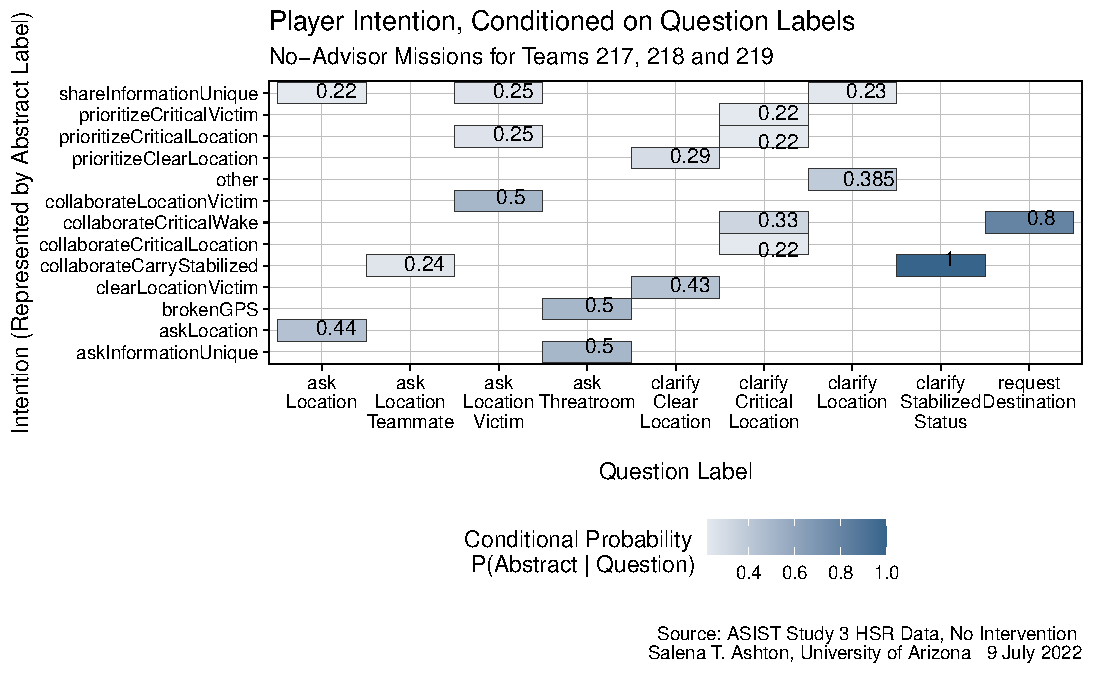
\includegraphics[width=0.6\textwidth]{../figures/abstractLabel_ConditionalProbability_STA.pdf}
    \caption{ }
\end{figure}


\begin{figure}[h!]
    \centering
    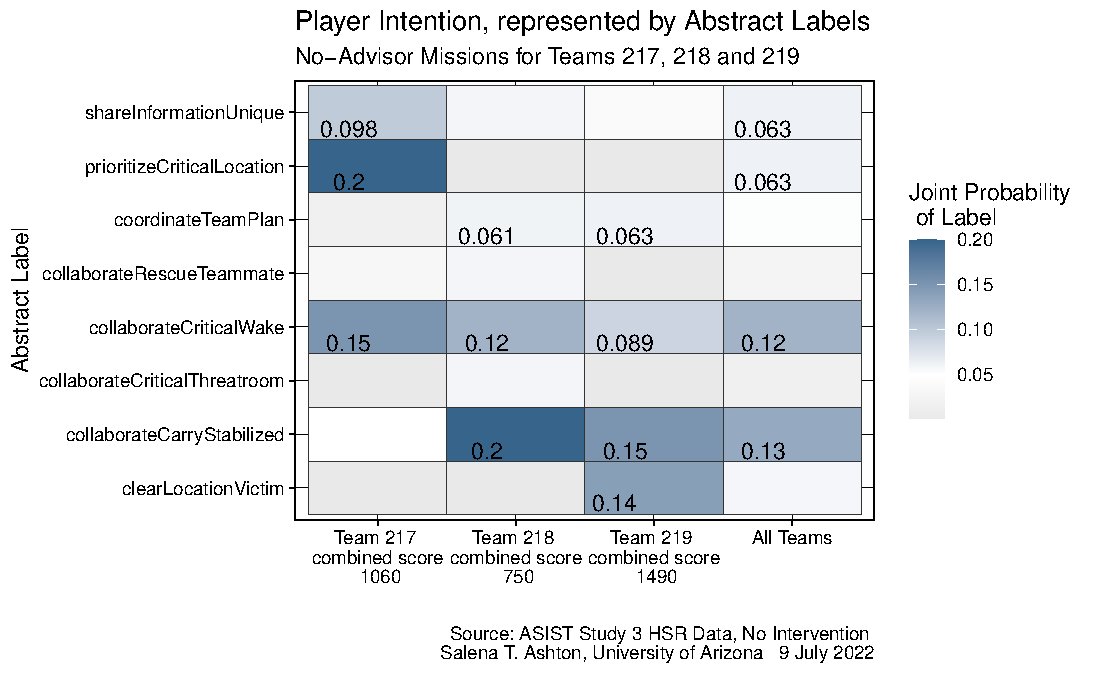
\includegraphics[width=0.6\textwidth]{../figures/abstractLabelProbability_STA.pdf}
    \caption{ }
\end{figure}


\begin{figure}[h!]
    \centering
    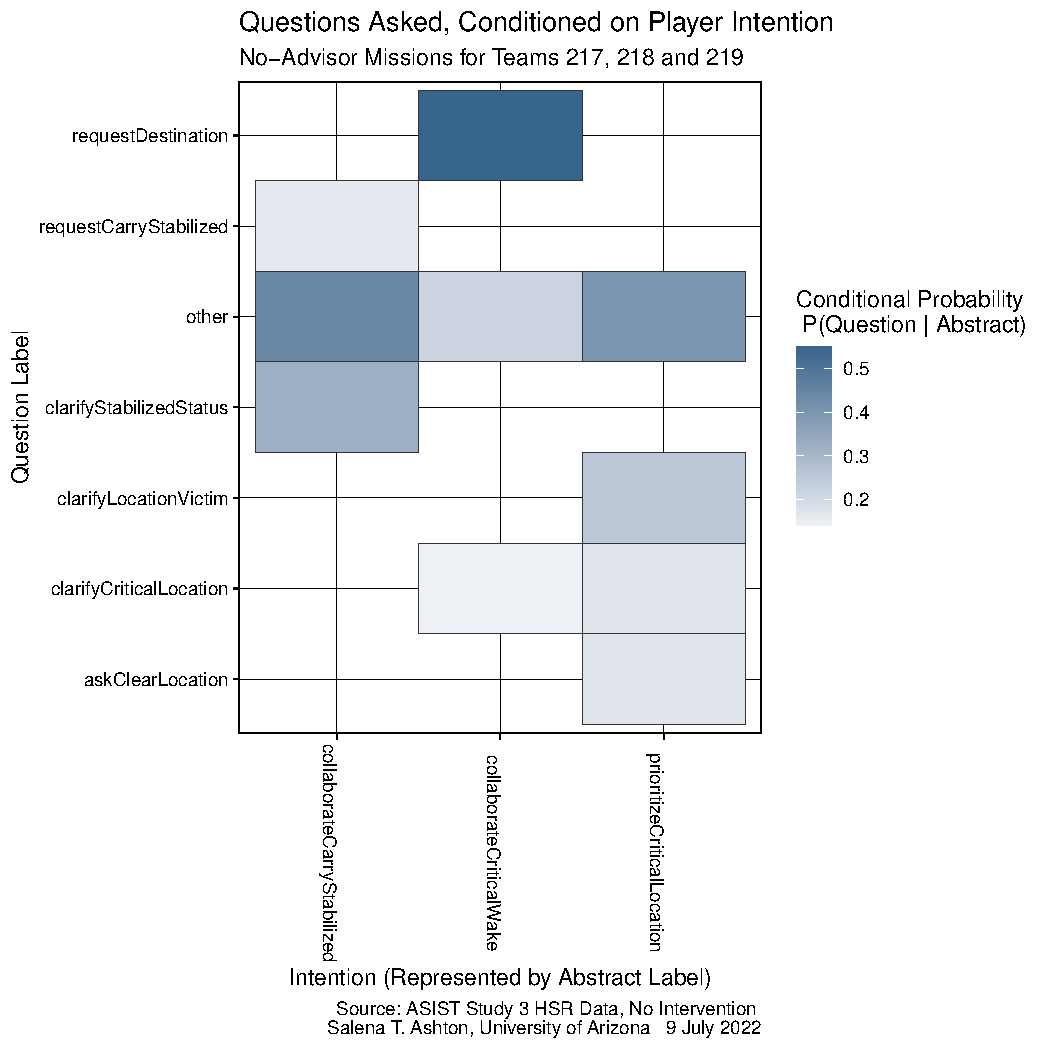
\includegraphics[width=0.6\textwidth]{../figures/questionLabel_ConditionalProbability_STA.pdf}
    \caption{ }
\end{figure}

\begin{figure}[h!]
    \centering
    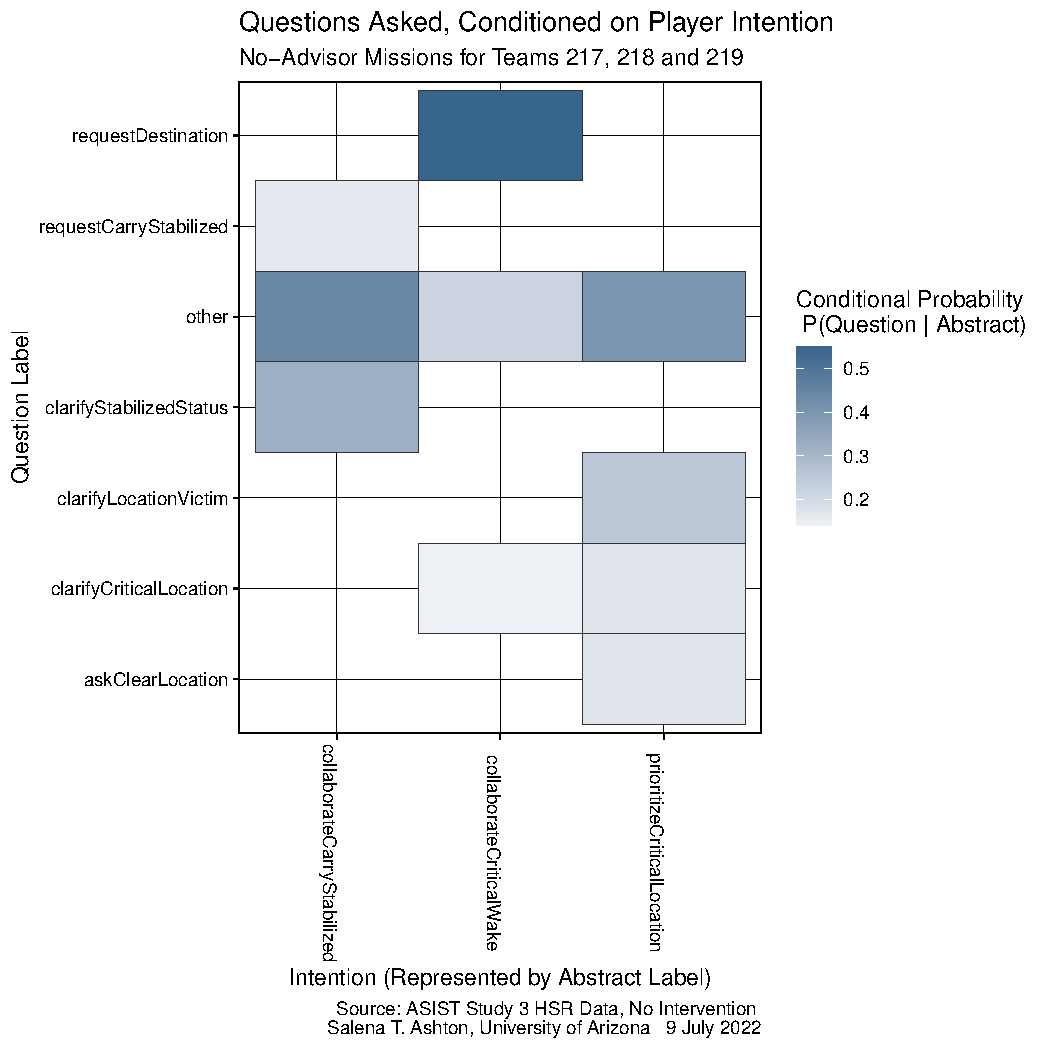
\includegraphics[width=0.6\textwidth]{../figures/questionLabel_ConditionalProbability_STA.pdf}
    \caption{ }
\end{figure}




\begin{figure}[h!]
    \centering
    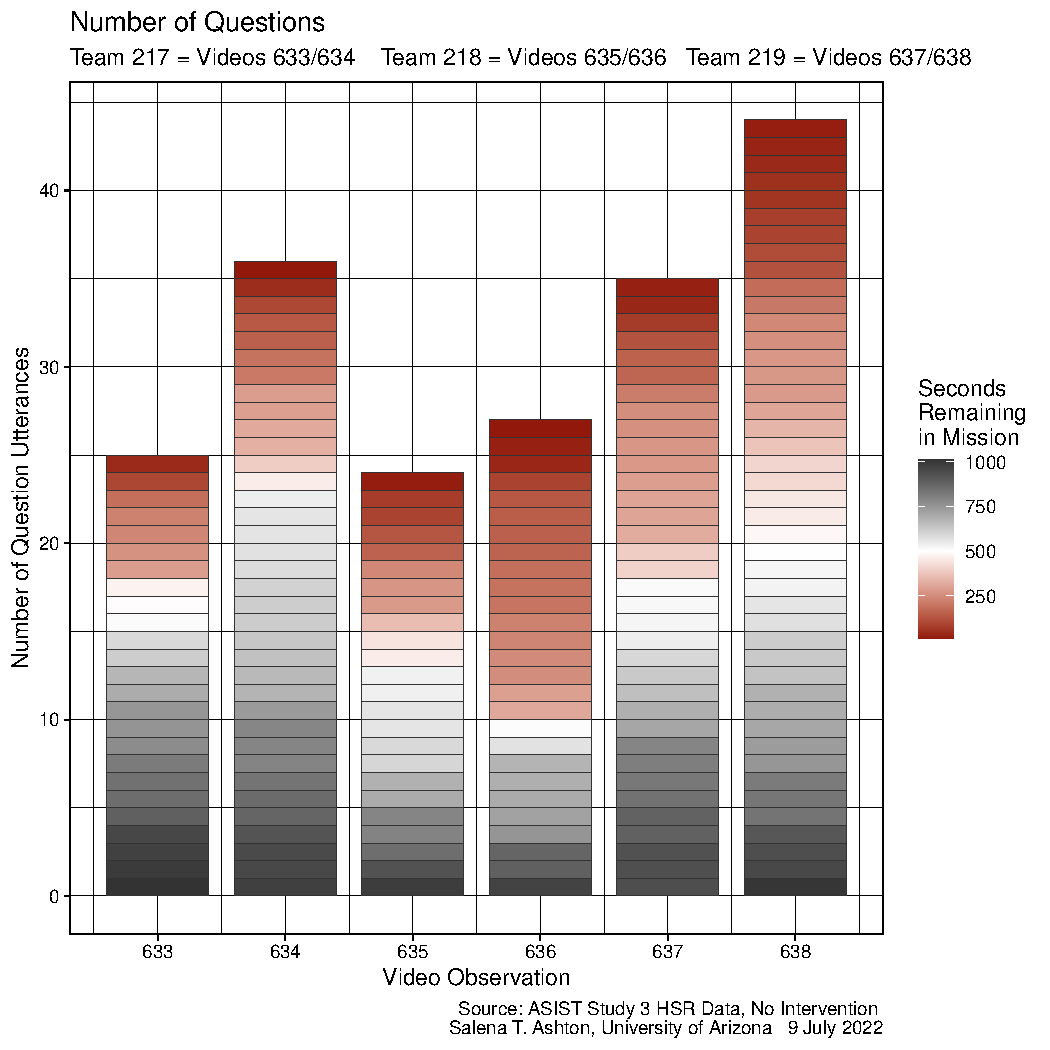
\includegraphics[width=0.6\textwidth]{../figures/QuestionTiming_STA.pdf}
    \caption{ }
\end{figure}

\clearpage












\subsection{Discussion and Future Research}
The ultimate goal of this work is two-fold: find enough evidence to warrant the continued investigation of question-asking through causal reasoning to discern player intention and to algorithmitize player intention from player utterance transcriptions of player without human annotator dependency. Due to the small sample size, we do not offer conclusive evaluations at this time. However, from these 12 video annotations, we \emph{can warrant} the further investigation of question-asking and inferred goals or intentions among human team players.

Key question phrases to give clues to ASI agents:
\begin{itemize}
    \item "If"
    \item
\end{itemize}



FUTURE RESEARCH:
\begin{itemize}
    \item knowledge engineering and representation of tasks, goals, and hidden intentions;  \emph{hierarchical task network} (HTN),
    \item scale for additional data
    \item Preliminary research can lead to additional annotation, quantitative analysis and generalized theories for ASI
    \item Compare and contrast theories that emerge from no-intervention data to high-intervention data
    \item Investigation into which data structures best capture human individual and team ToM
        \item Promised Future Investigation of RESEARCH QUESTIONS:
        \begin{itemize}
        \item How do spoken questions reveal another person’s plan or intent? 
    \item Can people listen to spoken questions and accurately decide if the other person's plan
        is simple, sequential, or hierarchical? Can the distinction between such
        structures improve predictive performance for Artificial Social
        Intelligence (ASI) agent intervention?
        \end{itemize}
        \item asdf
\end{itemize}



% End of stub Adarsh used for Repo
%%%%%%%%%%%%%%%%%%%%%%%%%%%%%%


\newpage

% To avoid spacious justification of the bibliography:
\raggedright
\bibliography{bibliography} % Name of bib file

\end{document}





